Hacer que las aplicaciones de Node.js estén listas para producción es probablemente el tema más oculto y omitido en la literatura de Node.js, pero es uno de los más importantes \cite{mardan}. Se requiere de un método estandarizado para que la efectividad del despliegue en el servidor de producción sea optima.

\subsubsection{Requisitos del servidor}

\begin{itemize}
  \item Servidor CentOS 7 con Git instalado.
  \item Al menos 512 Mb de RAM y 15 Gb de espacio libre en disco.
  \item Acceso de usuario root a través de SSH.
  \item Un nombre de dominio apuntado a la dirección IP del servidor (rosesland.app)
  % \item Editor de texto nano, puede instalarse con este comando:\\
  
  % \code{yum install nano}
\end{itemize}

\subsubsection{Servidor Privado Virtual}
Esta tecnología permite ejecutar las instancias de múltiples servidores en un servidor host físico de forma segura. Es un tipo de servidor de alojamiento web donde el alojamiento generalmente se realiza dividiendo un servidor físico principal en diferentes servidores virtuales múltiples. Cada uno de los servidores del sistema obtiene su propia parte de los recursos en función de los requisitos del cliente.
\vspace{0.8cm}

Este proyecto utiliza un servidor privado virtual (VPS) alojado en Digital Ocean, en donde debe decidir qué sistema operativo se desea, configurar el acceso SSH, crear un firewall, instalar los distintos lenguajes que necesita, etcétera. Para crear el VPS para el proyecto se accede a www.digitalocean.com y se crea una cuenta en Digital Ocean. Es necesario verificar la cuenta con una dirección de correo electrónico antes de poder crear un proyecto. Una vez verificada la dirección de correo electrónico, deberá un método de pago para el servicio. Al finalizar el registro y el modo de financiamiento se puede comenzar a configurar un servidor o Droplet. En Digital Ocean un Droplet es una máquina virtual simple y escalable. Con un costo de solo 5 dolares al mes, el plan básico es lo suficiente para mantener el proyecto en operación.
\vspace{0.8cm}

\begin{figure}[H]
  \centering
  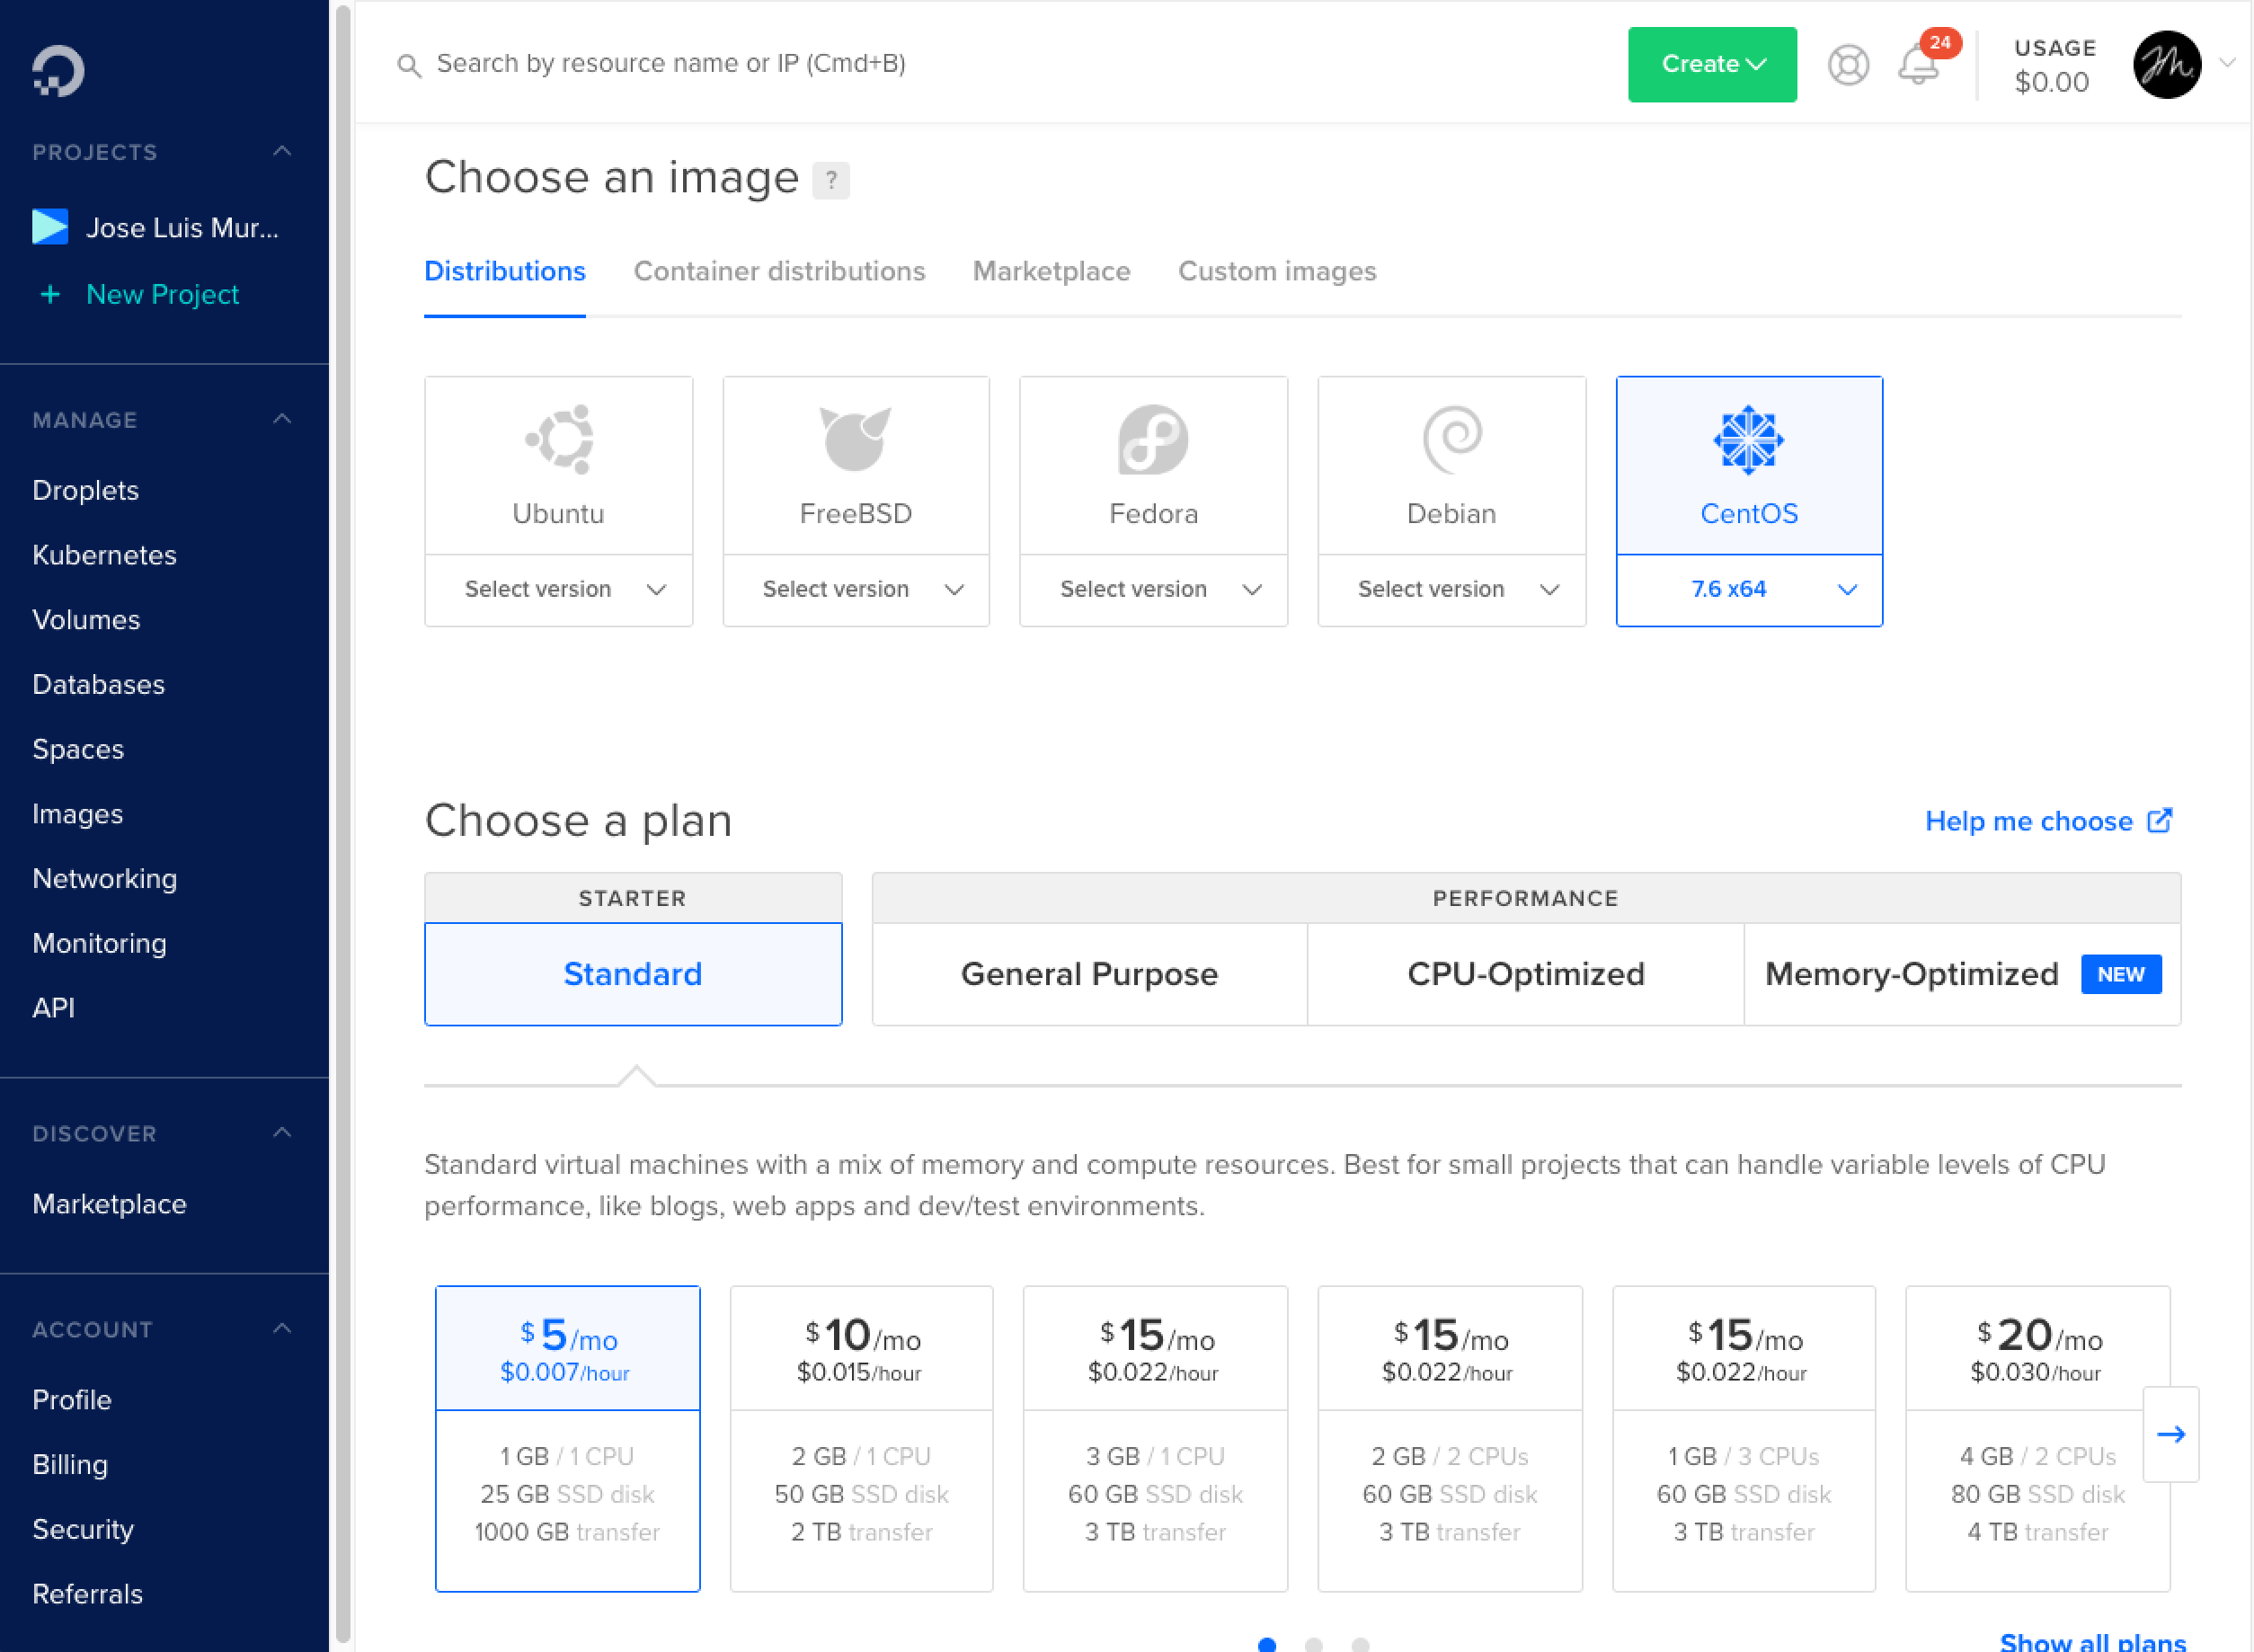
\includegraphics[width=1\textwidth]{digital-ocean}
  \caption{Configuración básica del servidor virtual privado.}
  \label{digital-ocean}
\end{figure}

Una vez que el servidor es creado, se recibe un correo electrónico de Digital Ocean. Este correo electrónico contiene los detalles de inicio de sesión para el servidor, en donde podremos conectarnos mediante SSH.
\vspace{0.8cm}

\subsection{Configurar despliegue automático con Git}
Al utilizar Git, el flujo de trabajo generalmente se dirige solo al control de versiones. Se tiene un repositorio local donde se trabaja y un repositorio remoto donde se mantiene todo sincronizado y se puede trabajar con un equipo y diferentes máquinas. Pero también es posible usar Git para mover una aplicación a producción \cite{vaccaro}.
\vspace{0.8cm}

\subsubsection{Configuración de repositorios}
Para poder empujar cambios a nuestro repositorio remoto se debe establecer la siguiente estructura:

\begin{itemize}
  \item Directorio publico del servidor: /var/www/rosesland.app
  \item Directorio del repositorio del servidor: /var/repo/site.git
\end{itemize}

Se inicia sesión en el VPS desde la consola de comandos y se ingresa lo siguiente:\\
\\
\code{cd /var}\\
\code{mkdir repo \&\& cd repo}\\
\code{mkdir site.git \&\& cd site.git}\\
\code{git init ---bare}\\

\code{---bare} significa que la carpeta no tendrá archivos fuente, solo el control de versiones.

\subsubsection{Git Hooks}
Los repositorios de Git tienen una carpeta llamada \code{hooks}. Esta carpeta contiene algunos archivos de muestra para conectar y realizar acciones personalizadas. La documentación de Git define tres posibles enlaces de servidor: \textit{pre-recepción}, \textit{post-recepción} y \textit{actualización}. Para este proyecto se necesita un `hook' para post-recepción, que se ejecuta cuando un `envío' está completamente terminado.
\vspace{0.8cm}

En el repositorio se encuentran algunos archivos y carpetas, incluida la carpeta \code{hooks}. Se accede a ella mediante el siguiente comando.\\
\\
\code{cd hooks}\\
\\
Se crea el archivo post-recepción escribiendo:\\
\\
\code{cat > post-receive}\\
\\
Al ejecutar este comando, se muestra una línea en blanco que indica que todo lo que escriba se guardará en este archivo. Se debe agregar lo siguiente:\\
\\
\code{\#!/bin/sh}\\
\code{git --work-tree=/var/www/rosesland.app --git-dir=/var/repo/site.git checkout -f}\\
\\
Al terminar, se presiona `control-d' para guardar. Para ejecutar el archivo, se necesita establecer los permisos adecuados usando:\\
\\
\code{chmod +x post-receive}\\
\\
El archivo post-recepción se examina cada vez que se completa un envío y coloca los archivos en \code{/var/www/rosesland.app}, esto permite actualizaciones directas del proyecto facilitando el mantenimiento de codigo y evitando la tarea de tener que conectarse al servidor para cargar los archivos manualmente.
\vspace{0.8cm}

En el repositorio local se necesita configurar la ruta del repositorio remoto. Se le dice Git que agregue un control remoto llamado `live':\\
\\
\code{git remote add live ssh://root@rosesland.app/var/repo/site.git}\\
\\
Con esto es posible empujar cambios en el repositorio al servidor remoto usando el alias `live':\\
\\
\code{git push live master}\\
\\
Con esto se le dice a Git que empuje al remoto `live' en la rama `master'.
\vspace{0.8cm}

\subsubsection{Despliegue Node.js en un entorno de producción}
